\section{Introduction}
\label{sec:maggie_introduction}

\newcommand\rvir{r_{\rm vir}}
\newcommand\vvir{v_{\rm vir}}

We show in the last chapter that the most used galaxy group algorithm that
is the FoF should be optimized against its linking lengths, and that it
depends on the scientific goal of the group catalog obtained. With these
limitations, it is clear why Bayesian methods appeared. Indeed, with our
knowledge of the galaxy formation and evolution processes, it is possible to
constrain better the galaxy grouping. With the FoF algorithm, galaxies are
selected in a pure geometrical way, and their formation history doesn't
matter in this selection, since only the over-density is relevant. With
Bayesian algorithms, it is possible to combine geometrical and physical
approaches. The history of galaxies is available by their observable
properties such as luminosity, stellar mass, morphology and is used to
assign galaxies to a group, in complement of the geometrical information
from the density. In particular, a galaxy can be rejected of a group
selected by density criterion if its properties don't reflect the history it
would have inside this group.

We already described Bayesian algorithms in
\bartrefchapter{galaxy_group_algorithms}, for example \citet{Yang+07} or
\citet{MunozCuartas+12}, where similar spatial methods to the FoF are
adopted, with priors as the density profile of galaxies inside halos to
constrain the assignation. But because of observational uncertainties, model
divergences, various incompletenesses\ldots, the extraction of groups from
observational data will always be affected these problems, and the galaxy
environment polluted by interlopers, creating biases in group
characteristics. This leads to bad modulation of galaxy properties with
their environment and a falsification of our understanding of intra-groups
physical processes.

Recently, with the improvement of computer capacities in terms of memory and
power, it becomes possible to include many priors in the computation, and to
use the most computation intensive applications of statistics. Since
interlopers will still be problematic, the new powerful computer era allowed
probabilities to describe the membership of galaxies in groups. Systematic
errors in galaxy surveys can be reduced or integrated in the grouping by
probabilities. For example, \citet{Liu+08} used a probabilistic FoF in
galaxy survey with photometric redshifts to avoid the uncertainties
inherent to this method. \citet{DominguezRomero+12} also used
responsibilities to improve the assignation of galaxies to groups and
reduce interlopers effect on their observable properties. In
\citet{Rykoff+14}, galaxies have their probabilities based on the group
richness estimations.

It seems that using probabilities to describe the membership inside galaxy
groups will inevitable, because of the systematic errors and biases presents
in the actual and future galaxy surveys. In particular, the modulation of
the galaxy properties with their environment that we want to extract from
galaxy group catalogues should be less biased by interlopers if we use
probabilities as a weight. Indeed, interlopers, even if they are still
present in the group membership, will have a low probability to pertain to
the group.

Here is the starting point of our galaxy group algorithm called MAGGIE\@:
Models and Algorithm for Galaxy Group, Interloper and Environment. We
combine our understanding from the galaxy formation, using various models,
to compute a probability for galaxies to belong to a peculiar group, and use
it in the algorithm for the group extraction. Then interloper effects should
be reduced in the characterization of the environment.

In the following sections, we will describe the algorithm and its

\section{Algorithm}
\label{sec:algorithm}

\subsection{Description}
\label{sub:maggie_description}

MAGGIE doesn't affect a galaxy to an
unique group, but it affects a probability for this galaxy to be in a group.
With this principle, a galaxy is assigned to more than one group. It's the
goal of MAGGIE\@: to obtain the properties of galaxy groups in statistical
and probabilistic senses. This allows users of catalogues generated by
MAGGIE to compute some properties of groups taking into account the fact
that a galaxy could not be assigned arbitrarily to one group with some
criteria of affectation. But the most important, it's that this probability
contains the information of being an interloper or not.

MAGGIE is organized in an iterative way in order to be self-consistent with
the data being analysed, as for learning algorithms. For this reason, we
will describe the implementation of the algorithm in different steps. In
what follows, we assume that we have a galaxy sample with
positions (right ascension RA, declination DEC), redshifts, stellar masses,
apparent magnitudes in a given band and absolute magnitudes. It's the
minimum set of data necessary.
%
\begin{enumerate}
    \item We first get some potentials groups in order to have a \emph{seed}
        in the iterative process. For this, we make an assumption: the most
        massive galaxies (in stellar mass) are potential group centers. In
        an other implementation, we use the luminosity of the central (the
        reason is explained in \note{Add the reference to section}). But,
        some intra-group physical process can lead to a false detection of
        the brightest galaxy as the central one \citep{Ebeling+13}. From the
        galaxy sample, we sort by decreasing stellar mass (or luminosity)
        all galaxies and we start with the most massive as centre of a
        potential group.

    \item\label{step:2} For all our potential groups, we need to get our
        potential members. We are just interested in the virial sphere of
        groups. Since the unique information on groups at this step is the
        central galaxy, we use its stellar mass. At first iteration, we use
        the relation between halo mass and central stellar mass from
        \citet{BCW+10}, we used other models later to see the influence of
        this choice (\note{Add reference to section}). For next iterations,
        we use the same relation, but learned from our previous iterations.
        We can estimate the virial radius of the group assuming
        that the halo mass corresponds to the virial mass. Then, we select
        all galaxies in a cone generated by an angular separation
        corresponding to the virial radius physical size at the group's
        redshift (the redshift of the central galaxy).

    \item With group membership, we compute galaxy probabilities to belong
        to it. The probability is computed assuming a density profile of
        galaxies in groups, and a velocity distribution. Considering that
        galaxies form in dark matter halos, the density profile of
        galaxies in groups must follow a NFW distribution \citep{NFW+97}
        which fit remarkably well the dark matter particles distribution in
        $\rm \Lambda$CDM simulations. The detailed computation of the
        probability is provided in \bartrefsection{probability}.

    \item We compute the weighted (by probability) stellar mass and
        luminosity of groups. For this we use a probability threshold to
        decide if a galaxy is associated to a group, i.e.\ if we take the
        galaxy for the estimation of the group stellar mass and luminosity.
        This parameter will be optimized by tests. The way of computing this
        properties for a group is the following: we sum, using the
        probability weights, luminosities and stellar masses of galaxies
        that have an absolute magnitude less than the limit magnitude
        defined by the sample, in order to be complete.

    \item Using the stellar mass of the central galaxy, we can estimate the
        halo mass of the group. We use the abundance matching technique
        which assumes that there is a one-to-one relation between the
        central stellar mass of the group and its halo mass. It allows to
        compare the cumulative distribution function (CDF) of the two
        masses. Indeed, with this assumption, the number of groups above a
        given central stellar mass is the same than the number of groups
        above the corresponding halo mass. If we consider a certain halo
        mass function, we can predict the halo mass of a group with a given
        central stellar mass by comparing the CDF of the data with that
        predicted by the halo mass function.

    \item With the halo mass found for group by this abundance matching, we
        go back to step~\ref{step:2} and recompute groups with the halo
        mass-central stellar mass relation previously obtained. This process
        goes until there is a convergence in the number of groups.
\end{enumerate}

\section{Probability}
\label{sec:probability}

The probability is one of the most important aspect of MAGGIE\@. Since the
observer study galaxy groups only in the projected phase space (hereafter
\emph{pps}), for defining the probability, we consider the location in
the \emph{pps} of the group with its projected radius $R$ and the
line-of-sight velocity $v_z$. The probability to be member of the halo or
not at a given location, is the number of cases where we are inside the halo
relatively to the total number of cases. The \emph{pps} density $g$ is this
definition of ``number of cases''. We can write our probability $p$ to be in
the halo as:
%
\begin{equation}
    \label{eq:probability}
    p \left(R, v_z\right)= \cfrac{g_h \left(R, v_z\right)}
    {g_h \left(R, v_z\right) + g_i \left(R, v_z\right)}
\end{equation}
%
where $g_h$ is the projected density inside the group and $g_i$ is the
background density, i.e.\ the interloper density.

In \bartrefsubsection{general_case}, we describe how to compute the
probability with a general density profile and then in
\bartrefsubsection{analytical_forms} some analytical forms
available with some models.

\subsection{General case}
\label{sub:general_case}

To compute the projected density of galaxies in the halo we have to assume some
models for their phase space distribution. So we use the distribution function
$f$ of the system:
%
\begin{equation}
    f\left(\textbf{r},\textbf{v}\right)\dd\textbf{r}\dd\textbf{v}
    =\rho\left(r\right)\dd{x}\dd{y}\dd{z}
    h\left(\textbf{v}\right)
    \dd v_r\dd v_\theta\dd v_\phi=
    \dd^6 N
\end{equation}
%
where $h\left(\textbf{v}\right)$ is the velocity distribution of galaxies in
the halo.

If we consider the line of sight as the axe of cylindrical coordinates, we
can write:
%
\begin{equation}
    f\left(\textbf{r},\textbf{v}\right)\dd\textbf{r}\dd\textbf{v}=
    \rho\left(r\right)R\dd{R}\dd\phi\dd{z}h\left(\textbf{v}\right)
    \dd{v_r}\dd{v_\theta}\dd{v_\phi}
\end{equation}

By definition, the projected phase space density is just the number $N$ of
galaxies with their \emph{pps} coordinates in the ring defined by the range
$R+\dd R$ and $v_z+\dd v_z$.
%
\begin{equation}
    g_h \left(R, v_z\right)2\pi R \dd R \dd v_z = \dd^2 N
\end{equation}

We can see that $r^2=z^2+R^2$, so $\dd{z}=r/\sqrt{r^2-R^2}\dd{r}$.
Now, to have the projected density on the sphere, we just need to integrate
over the line of sight and angles:
%
\begin{equation}
    \label{eq:intfunc}
    \int_0^{2\pi}\int_{z=-z_{\max\left(r\right)}}^{z_{\max\left(r\right)}}
    f\left(\textbf{r},\textbf{v}\right)\dd\textbf{r}
    \dd{\textbf{v}}=2\int_{r=R}^{r_{\mathrm{vir}}}2\pi
    \frac{r\rho\left({r}\right)}{\sqrt{r^2-R^2}}{R}\dd{R}\dd{r}
    {h\left({\textbf{v}}\right)}\dd{v_r}\dd{v_\theta}\dd{v_\phi}
\end{equation}

We need to integrate on the velocities too in order to get the line-of-sight
component, and retrieve the pps. For velocities, we make a transformation of
coordinates: we pass to spherical coordinates to the coordinates defined in
XX\@. The rotation matrix between two coordinates system is:
\begin{equation}
    \begin{pmatrix}
        v_r \\
        v_\theta \\
        v_\phi \\
    \end{pmatrix}
    =
    \begin{pmatrix}
        \cos\theta & \sin\theta & 0 \\
        \sin\theta & \cos\theta & 0 \\
        0 & 0 & 1 \\
    \end{pmatrix}
    \begin{pmatrix}
        v_z \\
        v_1 \\
        v_\phi \\
    \end{pmatrix}
\end{equation}
%
so the Jacobian of the transformation is unity:
%
\begin{equation}
    \label{eq:intintfunc}
    \int_0^{2\pi}\int_{z=-z_{\max\left(r\right)}}^{z_{\max\left(r\right)}}
    \int_{-\infty}^\infty\int_{-\infty}^\infty
    f\left(\textbf{r},\textbf{v}\right)\dd\textbf{r}\dd\textbf{v}=
    2\int_{r=R}^{r_{\mathrm{vir}}}2\pi
    \frac{r\rho\left(r\right)}{\sqrt{r^2-R^2}}R\dd{R}\dd{r}
    \tilde{h}\left(v_z\right)\dd{v_z}
\end{equation}
%
where $\tilde{h} \left(v_z\right) = \int_{-\infty}^\infty\int_{-\infty}^\infty
h \left(\textbf{v}\right)\dd v_1 \dd v_\Phi$

For simplifying the equations later, we used a normalization as in:
%
\begin{eqnarray}
    M(r)= &\int_0^r 4\pi x^2\rho \left(x\right)\dd x
        &=M_v{\overline{M}{(r/\rvir)}}\nonumber\\
    N(r)= &\int_0^r 4\pi x^2\nu \left(x\right)\dd x
        &=N_v{\overline{N}{(r/\rvir)}}\nonumber\\
    \rho\left(r\right)= &\cfrac{\dd M}{4\pi r^2\dd r}&=\frac{M_v}{4\pi \rvir^3}
        \overline\rho(r/\rvir)\nonumber\\
    \nu\left(r\right)= &\cfrac{\dd N}{4\pi r^2\dd r}&=
        \frac{N_v}{4\pi \rvir^3}\overline\nu (r/\rvir)\nonumber\\
\end{eqnarray}
%
where $a$ is the radius of slope -2 for the density profile in logarithm
scales, in other the radius where:
%
\begin{equation}
    {\left.\cfrac{\dd \log \rho \left(r\right)}{\dd \log r}\right|}_{r=a} = -2
\end{equation}

With this normalization, we can write:
%
\begin{equation}
    g_h \left(R, v_z\right) =\cfrac{M_v}{\rvir^2}
    \cfrac{1}{2\pi}
    \int_{R/\rvir}^1
    \cfrac{x\overline\rho \left(x\right)}{\sqrt{x^2 -
    {\left(R/a\right)}^2}}\dd x \widetilde{h} \left(v_z\right)
\end{equation}

The density of interlopers is extracted from \citet{MBM+10} where:
%
\begin{equation}
    g_i\left(R,v_z\right)=\undemi g_i\left(R,|v_z|\right)=
    \undemi\left(A
        \exp\left[-\undemi{\left(\frac{v_z}{\sigma_i}\right)}^2\right]
    +B\right)\frac{M_v}{\rvir^2 \vvir}=
    \widetilde g_i\left(R,v_z\right)\frac{M_v}{{r_{\rm{vir}}}^2 v_{\rm{vir}}}
\end{equation}

\subsection{Analytical forms}
\label{sub:analytical_forms}

In the following, we will refer to different equations of the
\bartrefappendix{profiles}.

If we assume that the halos are at the dynamical equilibrium, the velocity
distribution of galaxies should follow a Gaussian distribution. This
assumption can be discussed \citep{Beraldo+14}.

In this case, the velocity distribution can be written:
\begin{equation}
    h\left(\textbf{v}\right)=
    \frac{1}{{\left({2\pi}\right)}^{3/2}\sigma_{\theta}^2\sigma_r}
    \exp\left(-\undemi\left(\frac{v_r^2}{\sigma_r^2}+
    \frac{v_{\theta}^2+v_{\phi}^2}{\sigma_{\theta}^2}\right)\right)
\end{equation}
%
assuming that we split the three components of the velocity into three
independent velocity distributions. We can transform:
%
\begin{equation}
    \label{eq:poly}
    \left(\frac{v_r^2}{\sigma_r^2}+\frac{v_{\theta}^2+
    v_{\phi}^2}{\sigma_{\theta}^2}\right) =
    a v_z^2 + b v_1^2 + c v_\phi^2 + 2 v_z v_1 d
\end{equation}
%
for the coordinate system defined in\note{Add figure for the system}
with:
%
\begin{eqnarray}
    a&=&\left(\frac{\cos^2\theta}{\sigma_r^2}+
        \frac{\sin^2\theta}{\sigma_\theta^2}\right)\nonumber\\
    b&=&\left(\frac{\cos^2\theta}{\sigma_\theta^2}+
        \frac{\sin^2\theta}{\sigma_r^2}\right)\nonumber\\
    c&=&\frac{1}{\sigma_\theta^2}\nonumber\\
    d&=&\left(\frac{1}{\sigma_r^2}-\frac{1}{\sigma_\theta^2}\right)\nonumber\\
\end{eqnarray}
%
Putting \bartrefequation{poly} to a canonical form and integrating
\bartrefequation{intfunc} over $v_\phi$ and $v_1$ we get:
%
\begin{equation} \tilde{h}\left(v_z\right) = \frac{1}{\sqrt{2\pi}\sigma_z}
\exp\left(-\undemi{\left(\frac{v_z}{\sigma_z}\right)}^2\right) \end{equation}
%
since:
%
\begin{equation} \sigma_z^2 =
\sigma_r^2\left(1-\beta{\left(\frac{R}{r}\right)}^2\right) \end{equation}
%
and $\beta$ is the anisotropy profile $\beta=1-\sigma_\theta^2/\sigma_r^2$.

Finally, the projected density of galaxies in a halo is:
%
\begin{equation} g_h \left(R, v_z\right) =\cfrac{M_v}{\rvir^2}
    \cfrac{1}{2\pi}
    \int_{R/\rvir}^1
    \cfrac{x\overline\rho \left(x\right)}{\sqrt{x^2 -
    {\left(R/\rvir\right)}^2}}\frac{1}{\sqrt{2\pi}\sigma_z}
    \exp\left(-\undemi{\left(\frac{v_z}{\sigma_z}\right)}^2\right)\dd x
\end{equation}

If we work with velocities in units of the virial velocity $v_v$, i.e.\
$\hat{v_z}=v_z/v_v$, the ratio between the interloper and halo \emph{pps}
density is:
%
\begin{equation}
    \label{eq:gi_over_gh}
    \frac{g_i}{g_h}\left(R,v_z\right)=
    \frac{{\left(2\pi\right)}^{3/2}\hat{g}_i{(R/r_v,|v_z|/v_v)}}
        {\int_0^{\rm{acosh}\left(\frac{c}{x_R}\right)}
            \cfrac{\left(x_R\cosh{u}\right)\tilde\rho\left(x_R\cosh{u}\right)}
            {{\tilde\sigma}_z\left(x_R,x_R\cosh{u}\right)}
    \times\exp\left(-\undemi\frac{{\hat{v}_z}^2}
    {{\tilde\sigma}_z^2\left(x_R,x_R\cosh{u}\right)}\right)\dd u}
\end{equation}
%
where we used the transformations $x=x_R\cosh u$ and $x_R=R/\rvir$, to obtain a
better convergence for the numerical integration. Simplifications are coming
from the expression of the virial velocity $v_v^2=\cfrac{G M_v}{r_{\rm vir}}$
and the dimensionless expression of the radial velocity dispersion deduced from
the Jeans equation (see \bartrefappendix{profiles}).

\subsection{Comparisons with simulations}
\label{sub:comparisons_with_simulations}

To test our computation of the probability, we compared our theoretical
expression with the dark matter particles from the simulations used in
\citet{MBM+10} to deduce the \emph{pps} density of interlopers. For this, a
selection of high masses dark matter halos was performed on the cosmological
simulation. Then, particles coordinates where translated to make the center of
the halo the origin of the simulation box. A fictive observer is placed in a
side of the box, and all observed coordinates in phase space are computed from
the observer point of view. The coordinates of all particles in the cone
defined by the observer and the radius of the halo are computed in units of the
virial radius and velocity. This allows to easily define a particle as an
interloper or not, with their three dimensional radial coordinate $r$. If in units
of the virial radius, $r\leqslant1$ means that the particle is belonging to the
halo, else it's an interloper. We can stack all the particles from all the
cones of each halo to create an unique halo, with numerous particles, used as a
test case for our models and to estimate the interloper \emph{pps} density.

In \bartreffigure{probabilities}, we show the contours of the probability to
belong to the halo (in gray for the simulation, in black for our model from the
\bartrefequation{gi_over_gh}) in the \emph{pps}. For this model, we used a
Gaussian velocity distribution of particles in the halo, with the anisotropy
from \citet{ML+05} that fit the anisotropy profile of dark matter particles,
and we assumed a NFW density profile. Moreover, we assume that the
characteristic radius of the anisotropy of \citet{ML+05} is equal to the $a$
radius at which the slope of the density profile is -2. The theory fits
relatively well the data from the cosmological simulation, excepted for high
values of the line-of-sight velocity.
%
\begin{figure}[ht]
    \centering
    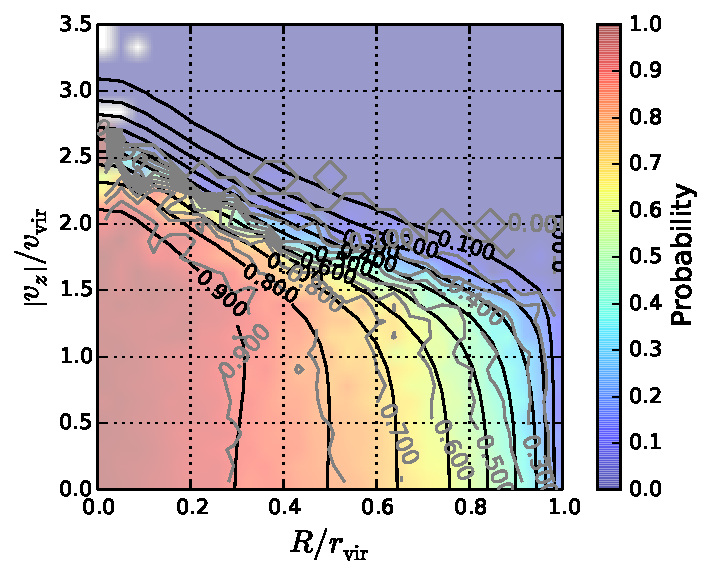
\includegraphics[width=0.6\linewidth]{figures/maggie/probabilities.pdf}
    \caption{The probability contours from the simulation of Borgani (put a
        reference) and our model. In \emph{gray} the contours obtained with
        particles from the cosmological simulation, and in \emph{black} the
        theoretical expectation from \bartrefequation{gi_over_gh}. The color
        scale reflects the probability from the simulation. The theoretical
        probability agree with the cosmological simulation except for high
        velocities along the line-of-sight, in part explained by the lack of
        particles with such velocities, giving a bad constraint for the
        probability to be in the halo from the simulation.
\label{fig:probabilities}}
\end{figure}

\remark{%
    We can first think that the observed discrepancies in
    \bartreffigure{probabilities} are the consequence of a bad choice for the
    ratio $a/b$ (see \bartrefappendix{profiles}) or for the concentration, but
    changing this values doesn't reduce them. The contours for the simulation
    seem to show a cut-off in the line-of-sight velocity dispersion for high
    velocities, like if the distribution is truncated above a given velocity. A
    functional form with such a property is the generalization of the Gaussian
    called the $q$-Gaussian or Tsallis distribution. Assuming such a velocity
    distribution, the computation of the probability involves several
    integrals, which is CPU time consuming. Instead, we can fit a $q$-Gaussian
    on the line-of-sight velocity distribution from the simulation and
    incorporate it in the probability computation. But unfortunately, this
    doesn't solve the problem. It seems that the number of particles with high
    velocities is too low to correctly define the probability to be in the
    virial sphere of the halo, and to compare it to theoretical expectations.
}

\section{Results on mock catalogue}
\label{sec:results_on_mock_catalogue}

\section{Application to SDSS}
\label{sec:application_to_sdss}


% vim: set tw=79 ft=tex:
